% !TEX root = webmatematik.tex

\section{Multipel regression}

\subsection{Introduktion}
Fra simpel \href{http://www.webmatematik.dk/lektioner/matematik-b/regression}{lineær regressions} analyse ved vi, hvordan man med \href{http://www.webmatematik.dk/lektioner/matematik-b/regression}{mindste kvadraters metoden} bestemmer den lineære funktion, som bedst passer til en række observationer i 2D planen.

Vi har altså her observationer \((y_i, x_i)\) for \(i=1,\ldots,n\) og ønsker at bestemme konstanterne \(a\) og \(b\) på en sådan måde, at den lineære funktion
\begin{displaymath}
  y = a + b x
\end{displaymath}
ligger så tæt på alle observationer \((y_i, x_i)\) som muligt.

Verden er dog sjældent så simpelt indrettet, at man kan beskrive en \textit{afhængig} variabel \(y\) med kun en enkelt \textit{forklarende} variabel \(x\).

Multipel regression er en udvidelse af simpel regression, hvor vi i stedet for en enkelt for\-kla\-ren\-de variabel har to eller flere forklarende variable. For\-kla\-ren\-de variable kaldes til tider også for \textit{kovarianter}.

\subsection{Model}
Vi har \(n\) observationer \(y_i,x_{1,i},x_{2,i},\ldots,x_{p,i}\) hvor \(i=1,\ldots,n\) og ønsker at bestemme konstanter \(b_0,b_1,b_2,\ldots,b_p\), så funktionen
\begin{displaymath}
  y = b_0 + b_1 x_1 + b_2 x_2 + \cdots b_p x_p
\end{displaymath}
ligger så tæt på alle punkterne \(y_i,x_{1,i},x_{2,i},\ldots,x_{p,i}\) som muligt.

Bemærk, at der nu er et dobbelt indeks på \(x\)'erne. Det er nødvendigt, da vi nu istedet for en enkelt forklarende variabel, har \(p\) forklarende variable. Så når vi skriver

\begin{displaymath}
  x_{ji}, \quad j=1,\ldots,p \textrm{ og } i=1,\ldots,n
\end{displaymath}
er der tale om den \(j\)'te forklarende variable for den \(i\)'te observation.

Koefficienter bliver normal fundet (estimeret) ved brug af mindste kvadrater metoden, dvs man vælger \(b_0, b_1, \ldots , b_p\)  således at udtrykket
\begin{displaymath}
  RSS =\sum^n_{i=1} {\big(y_i - b_0 - b_1 x_{i1} - b_2 x_{i2} - \cdots - b_p x_{ip} \big)}^2
\end{displaymath}
minimeres. RSS er engelsk for Residuals Sum of Squares. Dette er samme fremgangsmetode som kendes fra simpel lineær regression. Ofte omtales \(b_0\) som skæringen og de øvrige \(b\)'er som hældningen.

Formlen for koefficienterne \(b_0,b_1,b_2,\ldots,b_p\) er noget mere kompliceret i det generelle tilfælde, så den springer vi over her. Men nedenfor viser vi et eksempel på, hvordan man kan bestemme koefficienter ved brug af Microsoft Excel.

\subsection{Visualisering af løsningen}
I tilfældet med simpel regression bestemmer vi en ret linie som passer bedst til observationerne. Det er umuligt at visualisere multipel regression i det generelle tilfælde. For det særlige tilfælde, hvor vi har to forklarende variable \(x_1\) og \(x_2\) og dermed modellen
\begin{displaymath}
  y = b_0 + b_1 x_1 + b_2 x_2
\end{displaymath}
så kan vi stadig visualisere løsningen. Vi kan tænke på observationerne \((x_{1i}, x_{2i}, y_i), i=1,\ldots,n\) som punkter i rummet, dvs i 3D koordinatsystemet med akser \(X_1, X_2\) og \(Y\).
\begin{center}
\missingfigure[figwidth=12cm]{}
\end{center}
Løsningen er nu ikke længere en ret linie, men derimod den plan som ligger tættest på alle punkterne.

\subsection{Prognoser}
Hvis koefficienterne \(b_0,b_1,b_2,\ldots,b_p\) er kendt, kan vi bruge formlen
\begin{displaymath}
\hat{y} = b_0 + b_1 x_1 + b_2 x_2 + \cdots + b_p x_p
\end{displaymath}
til at forudsige
hvad bruger vi regression til - forudsige

\subsection{Eksempel}
Lad os se på et (simplificeret) eksempel på multipel regressionsanalyse. Eksemplet er hentet fra opgaven ``Prisdannelse på ejerlejligheder i København'' af Vibeke Stål og Anne Melvej Stennevad. Forfatterne undersøger, om der er en lineær sammenhæng mellem prisen på ejerlejligheder i København og en række faktorer såsom fx rente og byggeomkostninger.

\begin{displaymath}
  pris = b_0 + b_1 * byggeomkostninger + b_2 * renteniveau
\end{displaymath}

Hvordan bestemmer man \(b_0, b_1\) og \(b_2\) hvis vi har observationer som vist her i Excel
\begin{center}
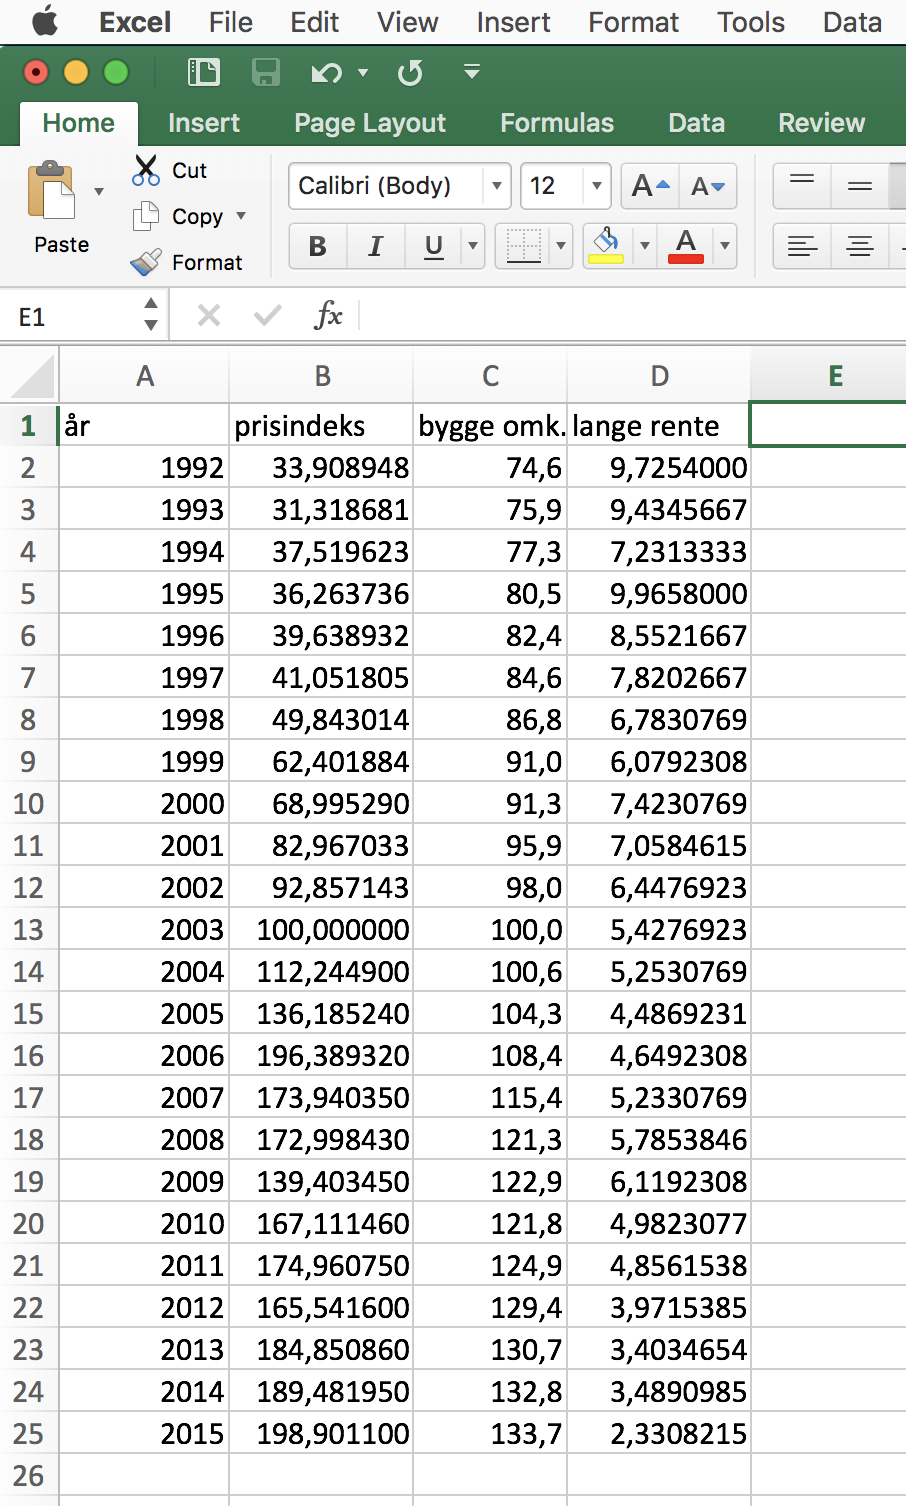
\includegraphics[height=12cm]{excel1.JPG}
\end{center}
I menuen under ``Tools'' finder man ``Data Analysis''\footnote{hvordan installerer man data analysis indsæt fodnote}
\begin{center}
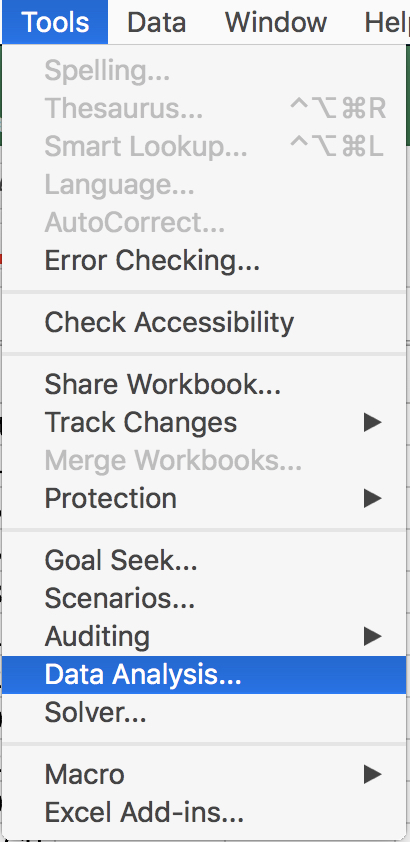
\includegraphics[height=8cm]{menu.JPG}
\end{center}
og dernæst fås en oversigt over de forskellige analyseværktøjer. Vælg ``Regression''
\begin{center}
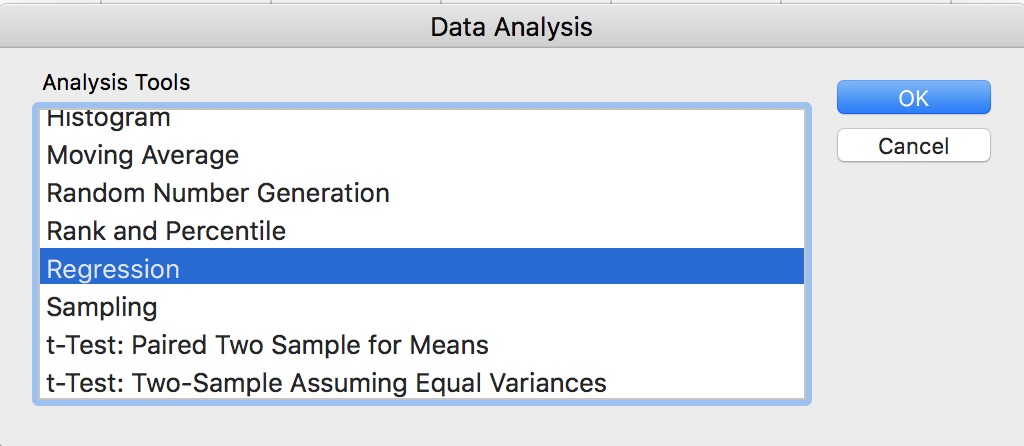
\includegraphics[height=4cm]{analysisTools.JPG}
\end{center}
Så dukker denne regression menu op
\begin{center}
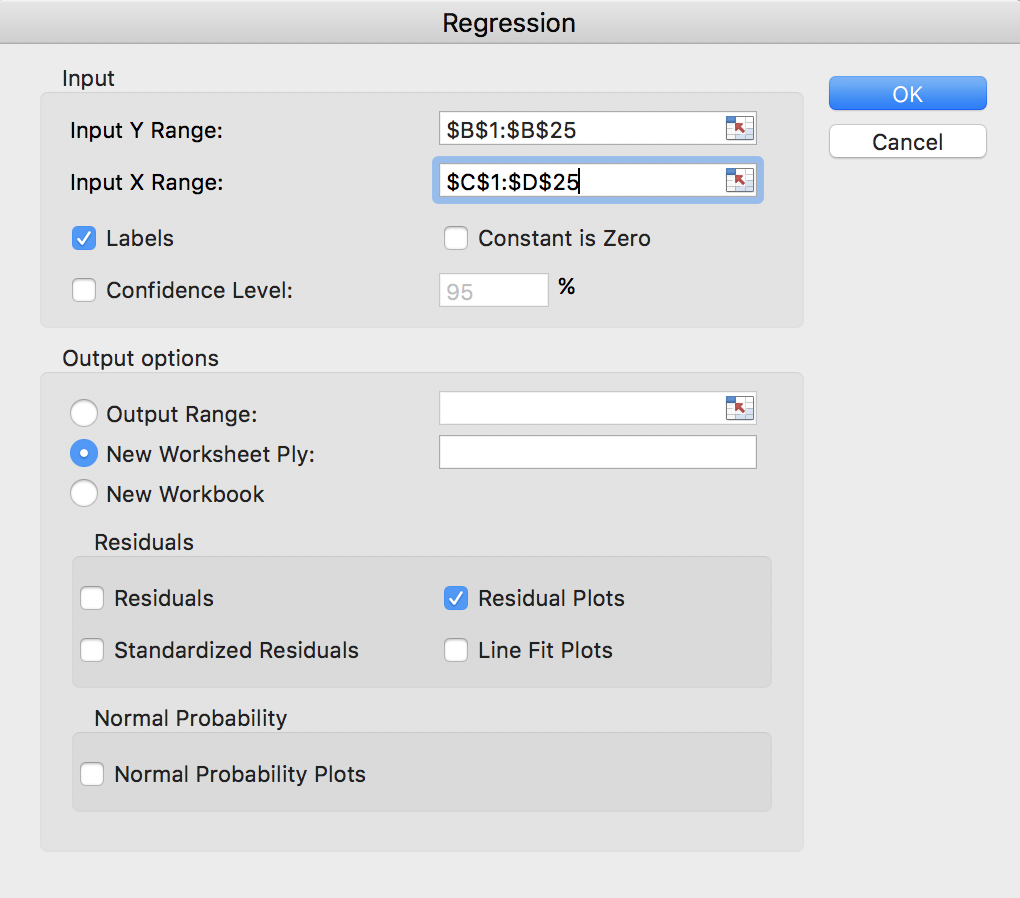
\includegraphics[height=9cm]{regression.JPG}
\end{center}
Her har vi som ``Input Y Range'' valgt kolonnen med prisindeks (inkl.\ overskriften). Dette er vores afhængige variable. Dernæst har vi som ``Input X Range'' valgt kolonnerne med data for byggeomkostninger og renter (igen inkl.\ overskrift). Ved at sætte kryds i ``Labels'' checkboksen fortæller vi Excel, at vores valg af inputdata indeholder overskrifter. Det gør det nemmere at læse resultaterne. Som det sidste vælger vi også ``Residual Plots''.

Som udgangspunkt bliver alle resultater placeret i en nyt sheet. Så er det lettere at slette dette sheet og begynde forfra, hvis man får behov for det.

Der er en masse output fra beregningen, men i første omgang fokuseres vi på tallene under overskriften ``Regression Statistics'':
\begin{center}
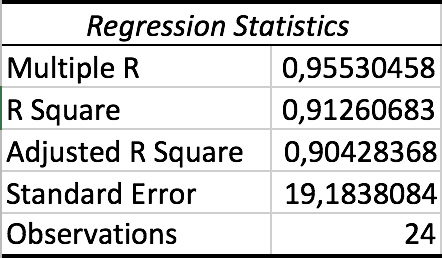
\includegraphics[height=4cm]{resultat.JPG}
\end{center}
hvor vi sætter fokus på Multiple R og R Square. På dansk kaldes disse to værdier for determinations- og korrelationskoefficienten.


\subsection{Korrelationskoefficienten}
Det er med Excel altid muligt at bestemme konstanterne \(b_0,b_1,b_2,\ldots,b_p\), så spørgsmålet er mere, om det giver mening at forsøge at modellere en lineær sammenhæng mellem en afhængig variable og en eller flere forklarende variable. Det kan korrelationskoefficienten hjælpe os med at afklare.



\subsubsection{Formel for korrelationskoefficient for 2 uafhængige variable}

\subsubsection{Fortolkning af korrelationskoefficient}

\begin{displaymath}
  R = \frac{\sqrt{r^2_{yx_1} + r^2_{yx_2} - 2r_{yx_1} r_{yx_2} r_{{x_1}x_2}}}{\sqrt{1 - r^2_{{x_1}x_2}}}
\end{displaymath}

sammenhæng til simpel regression. se led falde bort

\subsection{Determinationskoefficient}

kaldes også forklaringsgraden

\subsubsection{Formel}


\subsection{Residualplot}


\subsection{Konfidensinterval for parametre}




\subsection{brug din fornuft}
counterexample
anscombe
kig på graf

\subsection{model selection}

\subsection{adjusted \(R^2\)}


pas på med multicollinearity.

\subsubsection{Historie}


